\documentclass[tikz, border=10pt]{standalone}


\begin{document}


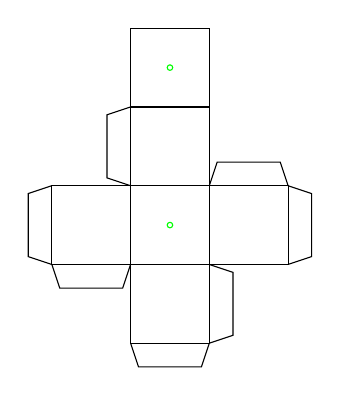
\begin{tikzpicture}[auto]
    \def\square#1#2{%
        \draw[xshift=#1cm, yshift=#2cm] (0,0) -- ++(1,0) -- ++(0,1) -- ++(-1,0) -- cycle;
    }

    \def\tab#1#2#3{
        \draw[xshift=#1cm, yshift=#2cm, rotate=#3] (0, 0) -- ++(0.1, 0.3) -- ++(0.8, 0) -- ++(0.1, -0.3);
    }

    % (1, -1, -1) -> (0, 0) 
    % (1, 1, 1) -> (1, 1) 
    \square{0}{0}
    % (1, 0, 0)
    \draw[green] (0.5,0.5) circle (1pt);

    % (1, -1, 1) -> (1, 0)
    % (-1, 1, 1) -> (2, 1)
    \square{1}{0}
    \tab{1}{1}{0}
    \tab{2}{1}{-90}

    % (-1, -1, -1) -> (0, -1)
    % (1, 1, -1) -> (1, 0)
    \square{0}{-1}
    \tab{1}{0}{-90}
    \tab{1}{-1}{180}

    % (-1, -1, -1) -> (-1, 0)
    % (1, -1, 1) -> (0, 1)
    \square{-1}{0}
    \tab{0}{0}{180}
    \tab{-1}{0}{90}

    % (1, 1, -1) -> (0, 1)
    % (-1, -1, 1) -> (1, 2)
    \square{0}{1}
    \tab{0}{1}{90}

    % (-1, 1, -1) -> (0, 2) 
    % (-1, -1, 1) -> (1, 3) 
    \square{0}{2}
    % (1, 0, 0)
    \draw[green] (0.5,2.5) circle (1pt);

\end{tikzpicture}

\end{document}